%-- Intro --%

\begin{tframe}{Introduction}

This method is based on \emph{T. Carvalho}, \emph{V. Schetinger et al. }works presented in [1] and [2].
\vspace{1cm}

\textbf{Mail goal}: finding image inconsistencies based on \textbf{illuminant estimation} in order to determine if an image has been \textbf{tampered} or not.

\begin{center}
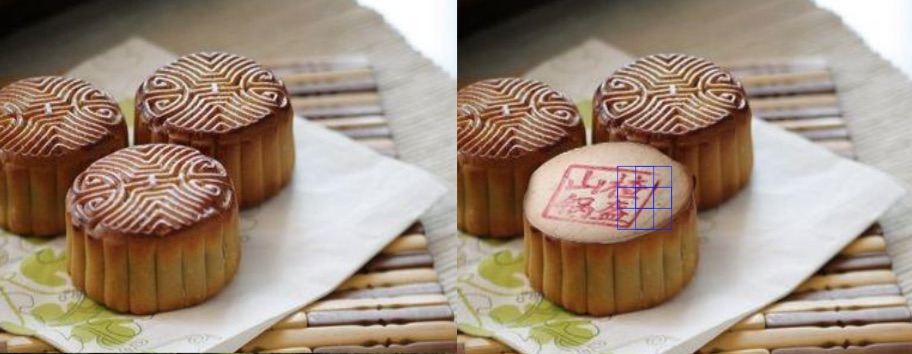
\includegraphics[width=0.6\textwidth]{images/cakes.jpg}
\end{center}

\end{tframe}

%-- Proposed method --%

\begin{tframe}{The proposed method}
\vspace{0.2cm}
\begin{enumerate}
\item \textbf{Illuminant Map} estimation
\vspace{0.2cm}
\begin{enumerate}
\item Generalized Grayworld Estimate (\textbf{GGE})
\vspace{0.2cm}
\item Inverse-Intensity Chromaticity (\textbf{IIC})
\vspace{0.2cm}
\end{enumerate}
\item \textbf{Statistical difference} between the IMs
\vspace{0.2cm}
\item Image \textbf{descriptor}
\vspace{0.2cm}
\item \textbf{Classification}
\end{enumerate}

\end{tframe}

\begin{tframe}{Illuminant Maps {\small [Schetinger \emph{et al.} 2016]}}
\vspace{0.1cm}
Extending previous work using different ways to use \textbf{combinations of different IMs}. It works on single ROIs.
\vspace{0.2cm}
\begin{minipage}{\textwidth}
\begin{columns}[T]
\begin{column}{0.5\textwidth}
\vspace{0.4cm}
\begin{small}
\begin{enumerate}
\item IM estimation using CGE and IIC
\item \textbf{Statistical difference}:
$$\vartheta = \frac{1}{q} \sum_{i = 1}^{q} \log (\| \lambda_i*(g_{GCE})^2 - \lambda_i*(f_{IIC})^2 \|)$$
\item Create \textbf{image descriptor} combining multiple eigenvalues
\item SVM classifier
\end{enumerate}

\end{small}
\end{column}
\begin{column}{0.4\textwidth}
\centering
\vspace{1.5cm}

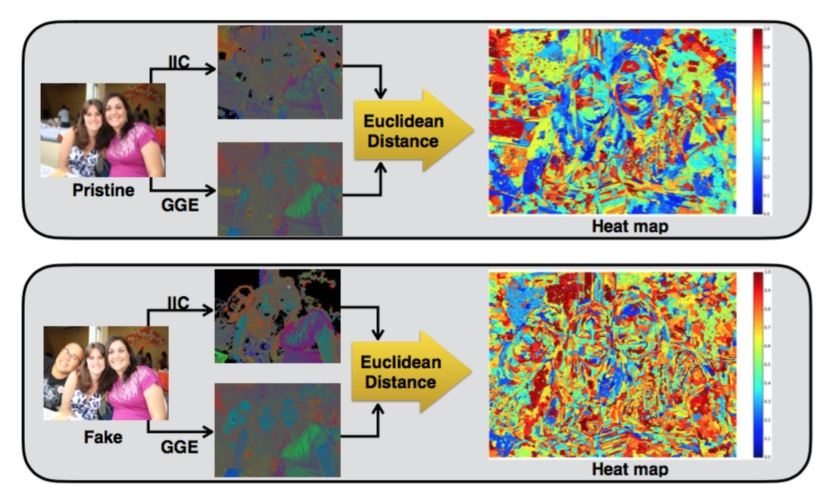
\includegraphics[width=\textwidth]{images/victor.jpg}
\end{column}
\end{columns}
\end{minipage}

\end{tframe}


